\section{The Cleaning Service}
\label{sec:cleaning}

This section presents cleaning module, which enables user to identify a certain kind of quality problems in RDF data and to handle these problems either  by removing all problematic triples (automatic cleaning using web service) or in interactive cleaning process using OpenRefine extension for RDF clenaing. 

The great majority of details regarding functionality as well as architecture of the cleaning module introduced in Deliverable 3.1~\cite{d3.1} and Deliverable 3.2~\cite{d3.2}, remains unchanged.
To keep the document short, we will not present them again. 
In this deliverable, we describe the changes and extensions that have been made in the resent period. 

The following improvements were performed:
\begin{itemize}
\item Integration of the Cleaning Web Service into OpenRefine extension
\item Implementation of user friendly interface for the cleaning  web service
\item Automatical creation of OpenRefine project from the given data file
\item Cleaning report is extended by statistics that summarize information about identifies quality problems. Respectively the QR Ontology which have been introduced in Deliverable 3.2~\cite{d3.2} were extended by the corresponding triples. 
\end{itemize}
A detailed description of the particular changes as well as design decisions and implementation details will be presented in the corresponding subsections.


\subsection{Cleaning Workflow}
The Cleaning Module desribed in the Deliverable 3.2~\cite{d3.2} consists of the two separate components - an OpenRefine extension to clean data in interactive way and the cleaning Web service for automatical cleaning.
In order to offer the user single entry point for the both cleaning way  we integrated the Web Service into OpenRefine extension whithout changing the functionalities of single components.
The updated workflow of the cleaning process including the both cleaning ways is presented in Figure \ref{fig:workflow}.


\begin{figure}[ht!]
\centering
\includegraphics[page=6,trim=0.5cm 0.5cm 0.5cm 0.5cm,clip,width=\textwidth]{figures/CleaningFigures.pdf}
\caption{Updated cleaning workflow}
\label{fig:workflow}
\end{figure}

The user starts cleaning by uploading his data and selecting the way he would like to clean data - interactive cleaning using OpenRefine or automatic cleaning by web services (Figure \ref{fig:entry}).
Several input data formats are supported, e.g.\todo{ @Ruslan please give here 2-3 different formats}.
By selecting OpenRefine a corresponding OpenRefine project will be created from the defined data set and user will be provided to the OpenRefine perspective.
Web service provide two different cleaning methods either generation of cleaning suggestions or deleting the problematic triples from the original data set.
More details about the different cleaning methods are presented in the section \ref{sec:openrefine} and \ref{sec:cleaningService}


\begin{figure}[ht!]
\centering
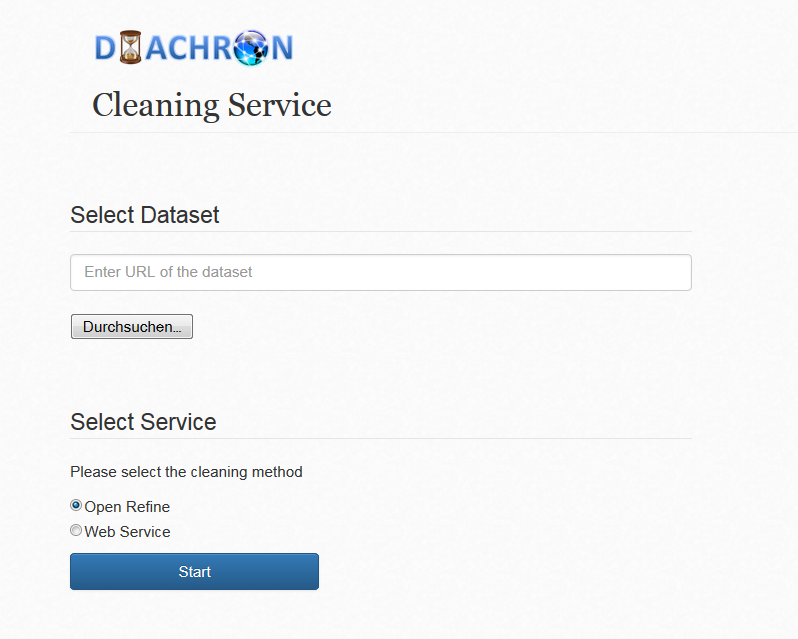
\includegraphics[width=11cm]{figures/CleaningStartPage.PNG}
\caption{User interface of Cleaning Module}
\label{fig:entry}
\end{figure}


\subsection{Cleaning with OpenRefine}
\label{sec:openrefine}

The mains steps of the cleaning workflow using OpenRefine initialy described in the Deliverable 3.2~\cite{d3.2} remains unchanged:
\begin{enumerate}
\item Project creation and representation of data set as `subject, predicate, object" table. In contrast to the previous cleaning module version the creation of OpenRefine project
occurs automaticaly in the back end from the input file defined by the user. 
\item Identification of quality problems. At this step the user define a set of metrics capturing his needs. The metric selection interface slightly changed. The updated version is shown in Figure \ref{fig:metric_selection}.
\item Generation of cleaning suggestions and interactive cleaning. In order to support the user in cleaning process for the UndefinedClass and UndefindedProperty problems we provide the user with concrete examples of classes or properties that could solve this problem. 
\todo{@Ruslan please provide a short description of the used method, reference to used diatnce metric and a screenshort of the OpenRefine with this suggestion}
\item Export cleaned data. The list of possible output formats were extended to the most popular formats : \todo{@Ruslan please list them} . We also implemented a user interface for this step (Figure \ref{fig:export}).
\end{enumerate}




\begin{figure}[ht!]
\centering
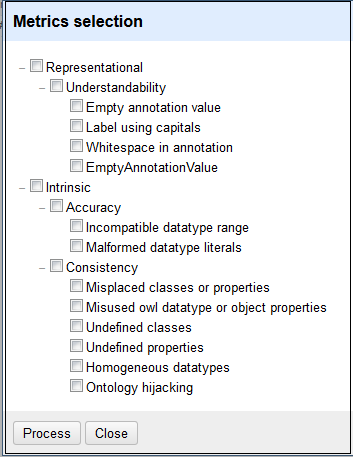
\includegraphics[width=6cm]{figures/MetricSelection.png}
\caption{Metric selection interface}
\label{fig:metric_selection}
\end{figure}



\begin{figure}[ht!]
\centering
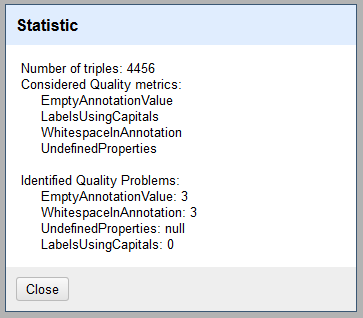
\includegraphics[width=8cm]{figures/statistics.png}
\caption{Cleaning statistics}
\label{fig:statistics}
\end{figure}


\begin{figure}[ht!]
\centering
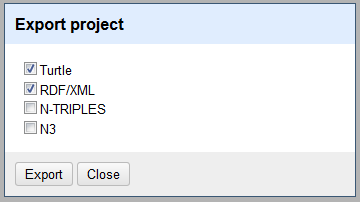
\includegraphics[width=6cm]{figures/export.png}
\caption{Export of cleaned data set in RDF format}
\label{fig:export}
\end{figure}



\todo{@Ruslan please fill the next sections}

\subsection{Technical Documentation}


\subsubsection{Architecture design}
UML diagramm
\subsubsection{Prerequisites}
updates ontologies,
new libraries

\subsubsection{How to install}
Install OpenRefine
Check out extension
Ruslan
\subsubsection{How to run}



%%% Local Variables: 
%%% mode: latex
%%% TeX-master: "D3.2"
%%% End: 
